\documentclass[12pt,a4paper]{article}
\usepackage[utf8]{vietnam}
\usepackage{amsmath,amssymb}
\usepackage{tabularx}
\usepackage{graphicx}
\usepackage{tikz}
\usetikzlibrary{calc,arrows.meta}
\usepackage{xcolor}
\usepackage{enumitem}
\usepackage{fancyhdr}
\usepackage[top=1.0cm, bottom=1.0cm, left=1.3cm, right=1.3cm]{geometry}
\usepackage[loigiai]{ex_test}
\SAOPTN{widthSA=2.6,heightSA=0.62}

\setlength{\headheight}{15pt}
\setlength{\parskip}{1pt}

\pagestyle{fancy}
\fancyhf{}
\rhead{\textit{Lời giải chi tiết -- Đề số 11}}
\lhead{\textit{Bộ đề ôn tập Giữa học kì I -- Toán 7}}
\cfoot{\thepage}

\begin{document}

\begin{center}
\textbf{\Large HƯỚNG DẪN CHẤM VÀ LỜI GIẢI CHI TIẾT}\\
\vspace{1mm}
\textbf{\large MÔN: TOÁN 7 -- ĐỀ SỐ 11}
\end{center}
\vspace{2mm}

\noindent\textbf{\large PHẦN I. CÂU TRẮC NGHIỆM NHIỀU PHƯƠNG ÁN LỰA CHỌN}

\vspace{1mm}
\begin{ex}
So sánh hai số hữu tỉ $x = -\dfrac{2}{5}$ và $y = \dfrac{-3}{13}$ ta được kết quả:
\choice
{$x > y$}
{\True $x < y$}
{$x = y$}
{$x \ge y$}
\loigiai{
Quy đồng mẫu số hai phân số với mẫu số chung là $65$ ta được $x = -\dfrac{26}{65}$ và $y = -\dfrac{15}{65}$. Do $-26 < -15$ nên $-\dfrac{26}{65} < -\dfrac{15}{65}$, suy ra $x < y$.
}
\end{ex}

\begin{ex}
Tia $Ot$ nào trong các hình dưới đây là tia phân giác của góc $xOy$?
\begin{center}
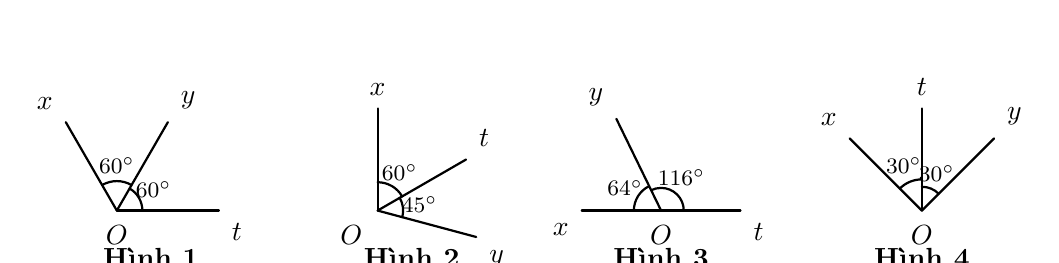
\begin{tikzpicture}[scale=0.72, line cap=round, line join=round]
    % Hình 1
    \begin{scope}[shift={(0,0)}]
        \coordinate (O) at (0,0);
        \coordinate (t) at (1.8,0);
        \coordinate (y) at (60:1.8);
        \coordinate (x) at (120:1.8);
        \draw[thick] (O) -- (t) node[below right=1pt] {$t$};
        \draw[thick] (O) -- (y) node[above right=1pt] {$y$};
        \draw[thick] (O) -- (x) node[above left=1pt] {$x$};
        \node[below=2pt] at (O) {$O$};
        \draw[thick] (O) ++(0:0.45) arc (0:60:0.45);
        \node[font=\footnotesize] at (30:0.75) {$60^\circ$};
        \draw[thick] (O) ++(60:0.52) arc (60:120:0.52);
        \node[font=\footnotesize] at (90:0.8) {$60^\circ$};
        \node[below=8pt] at (0.6,-0.1) {\textbf{Hình 1}};
    \end{scope}

    % Hình 2
    \begin{scope}[shift={(4.6,0)}]
        \coordinate (O) at (0,0);
        \coordinate (x) at (90:1.8);
        \coordinate (t) at (30:1.8);
        \coordinate (y) at (-15:1.8);
        \draw[thick] (O) -- (x) node[above=1pt] {$x$};
        \draw[thick] (O) -- (t) node[above right=1pt] {$t$};
        \draw[thick] (O) -- (y) node[below right=1pt] {$y$};
        \node[below left=2pt] at (O) {$O$};
        \draw[thick] (O) ++(30:0.5) arc (30:90:0.5);
        \node[font=\footnotesize] at (60:0.78) {$60^\circ$};
        \draw[thick] (O) ++(-15:0.45) arc (-15:30:0.45);
        \node[font=\footnotesize] at (8:0.75) {$45^\circ$};
        \node[below=8pt] at (0.6,-0.1) {\textbf{Hình 2}};
    \end{scope}

    % Hình 3
    \begin{scope}[shift={(9.6,0)}]
        \coordinate (O) at (0,0);
        \coordinate (t) at (1.4,0);
        \coordinate (x) at (-1.4,0);
        \coordinate (y) at (116:1.8);
        \draw[thick] (x) node[below left=1pt] {$x$} -- (t) node[below right=1pt] {$t$};
        \draw[thick] (O) -- (y) node[above left=1pt] {$y$};
        \node[below=2pt] at (O) {$O$};
        \draw[thick] (O) ++(0:0.4) arc (0:116:0.4);
        \node[font=\footnotesize] at (58:0.68) {$116^\circ$};
        \draw[thick] (O) ++(116:0.48) arc (116:180:0.48);
        \node[font=\footnotesize] at (148:0.75) {$64^\circ$};
        \node[below=8pt] at (0,-0.1) {\textbf{Hình 3}};
    \end{scope}

    % Hình 4
    \begin{scope}[shift={(14.2,0)}]
        \coordinate (O) at (0,0);
        \coordinate (t) at (90:1.8);
        \coordinate (x) at (135:1.8);
        \coordinate (y) at (45:1.8);
        \draw[thick] (O) -- (t) node[above=1pt] {$t$};
        \draw[thick] (O) -- (x) node[above left=1pt] {$x$};
        \draw[thick] (O) -- (y) node[above right=1pt] {$y$};
        \node[below=2pt] at (O) {$O$};
        \draw[thick] (O) ++(45:0.42) arc (45:90:0.42);
        \node[font=\footnotesize] at (68:0.7) {$30^\circ$};
        \draw[thick] (O) ++(90:0.55) arc (90:135:0.55);
        \node[font=\footnotesize] at (112:0.85) {$30^\circ$};
        \node[below=8pt] at (0,-0.1) {\textbf{Hình 4}};
    \end{scope}
\end{tikzpicture}
\end{center}
\choice
{Hình 1}
{Hình 2}
{Hình 3}
{\True Hình 4}
\loigiai{
Quan sát Hình 4, tia $Ot$ nằm giữa hai tia $Ox, Oy$ và tạo với hai tia này hai góc bằng nhau $\widehat{xOt} = \widehat{tOy} = 30^\circ$. Do đó $Ot$ là tia phân giác của góc $xOy$.
}
\end{ex}

\begin{ex}
Chọn câu trả lời đúng:
\choice
{Hai góc đối đỉnh thì kề nhau}
{\True Hai góc đối đỉnh thì bằng nhau}
{Hai góc đối đỉnh có tổng số đo bằng $180^\circ$}
{Hai góc đối đỉnh có tổng số đo bằng $90^\circ$}
\loigiai{
Theo tính chất của hai góc đối đỉnh, hai góc đối đỉnh thì bằng nhau.
}
\end{ex}

\begin{ex}
Giá trị của biểu thức $\sqrt{16} - \sqrt{25}$ là:
\choice
{\True $-1$}
{$1$}
{$3$}
{$-9$}
\loigiai{
Ta có $\sqrt{16} = 4$ và $\sqrt{25} = 5$. Suy ra $4 - 5 = -1$.
}
\end{ex}

\begin{ex}
Lăng trụ đứng tam giác có:
\choice
{\True 5 mặt, 6 đỉnh, 9 cạnh}
{6 mặt, 6 đỉnh, 6 cạnh}
{3 mặt, 6 đỉnh, 6 cạnh}
{2 mặt, 6 đỉnh, 3 cạnh}
\loigiai{
Hình lăng trụ đứng tam giác có 2 mặt đáy và 3 mặt bên, tổng cộng 5 mặt. Số đỉnh là 6 và số cạnh là 9.
}
\end{ex}

\begin{ex}
\immini{
Cho hình lăng trụ đứng tam giác $ABC.A'B'C'$, các mặt bên của hình trên là những hình gì?
\choice
{Tam giác}
{Hình thoi}
{\True Hình chữ nhật}
{Hình bình hành}
}{
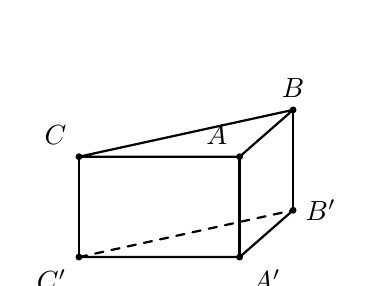
\begin{tikzpicture}[scale=0.85, line cap=round, line join=round]
    \coordinate (C) at (0, 1.5);
    \coordinate (A) at (2.4, 1.5);
    \coordinate (B) at (3.2, 2.2);
    \coordinate (C_prime) at (0, 0);
    \coordinate (A_prime) at (2.4, 0);
    \coordinate (B_prime) at (3.2, 0.7);

    \draw[thick] (C) -- (A) -- (B) -- (C);
    \draw[thick] (C) -- (C_prime);
    \draw[thick] (A) -- (A_prime);
    \draw[thick] (B) -- (B_prime);
    \draw[thick] (C_prime) -- (A_prime) -- (B_prime);
    \draw[thick, dashed] (C_prime) -- (B_prime);

    \filldraw[black] (C) circle (1.2pt) node[above left=1pt] {$C$};
    \filldraw[black] (A) circle (1.2pt) node[above left=1pt] {$A$};
    \filldraw[black] (B) circle (1.2pt) node[above=1pt] {$B$};
    \filldraw[black] (C_prime) circle (1.2pt) node[below left=1pt] {$C'$};
    \filldraw[black] (A_prime) circle (1.2pt) node[below right=1pt] {$A'$};
    \filldraw[black] (B_prime) circle (1.2pt) node[right=1pt] {$B'$};
\end{tikzpicture}
}
\loigiai{
Theo định nghĩa hình lăng trụ đứng, tất cả các mặt bên của hình lăng trụ đứng tam giác đều là hình chữ nhật.
}
\end{ex}

\begin{ex}
Trong các số sau, số nào là số vô tỉ?
\choice
{$\sqrt{\dfrac{25}{4}}$}
{\True $\sqrt{3}$}
{$\sqrt{(3{,}5)^2}$}
{$\sqrt{16}$}
\loigiai{
Các số $\sqrt{\dfrac{25}{4}} = \dfrac{5}{2}$, $\sqrt{(3{,}5)^2} = 3{,}5$ và $\sqrt{16} = 4$ đều là số hữu tỉ. Số $\sqrt{3} \approx 1{,}73205\ldots$ là số thập phân vô hạn không tuần hoàn nên là số vô tỉ.
}
\end{ex}

\begin{ex}
Với $a, b, c$ là ba số hữu tỉ bất kì, nếu $a - b = c$ thì:
\choice
{\True $a = b + c$}
{$a = -b + c$}
{$a = b - c$}
{$a = -b - c$}
\loigiai{
Áp dụng quy tắc chuyển vế, khi chuyển $-b$ từ vế trái sang vế phải ta đổi dấu thành $+b$: $a = c + b = b + c$.
}
\end{ex}

\begin{ex}
Điền cụm từ thích hợp vào chỗ chấm: “Một đường thẳng vuông góc với một trong hai đường thẳng song song thì nó cũng \dots với đường thẳng kia.”
\choice
{Song song}
{\True Vuông góc}
{Cắt nhau}
{Trùng nhau}
\loigiai{
Theo tính chất quan hệ giữa tính vuông góc và tính song song, đường thẳng đó cũng vuông góc với đường thẳng kia.
}
\end{ex}

\begin{ex}
Số thập phân $0{,}62313131\ldots$ dưới dạng thu gọn (có chu kì trong ngoặc) là:
\choice
{$0{,}(623)$}
{$0{,}(6231)$}
{\True $0{,}62(31)$}
{$0{,}623(13)$}
\loigiai{
Số thập phân có phần không tuần hoàn là $62$ và phần tuần hoàn lặp lại là $31$. Do đó viết gọn là $0{,}62(31)$.
}
\end{ex}

\begin{ex}
Trong các số $\dfrac{-9}{5}; \dfrac{-7}{-15}; 0{,}2; 0; \dfrac{-13}{2}; \dfrac{8}{5}$ có bao nhiêu số hữu tỉ dương?
\choice
{1}
{\True 3}
{2}
{4}
\loigiai{
Xác định các số lớn hơn $0$: $\dfrac{-7}{-15} = \dfrac{7}{15} > 0$; $0{,}2 > 0$; $\dfrac{8}{5} > 0$. Có tất cả 3 số hữu tỉ dương.
}
\end{ex}

\begin{ex}
Số đỉnh của hình hộp chữ nhật là:
\choice
{6}
{\True 8}
{10}
{12}
\loigiai{
Hình hộp chữ nhật có 4 đỉnh ở mặt đáy trên và 4 đỉnh ở mặt đáy dưới, tổng cộng có 8 đỉnh.
}
\end{ex}


\setcounter{ex}{0}
\noindent\textbf{\large PHẦN II. CÂU TRẮC NGHIỆM ĐÚNG SAI}

\vspace{1mm}
\begin{ex}
Xét tính đúng sai của các mệnh đề sau:
\choiceTF
{\True Tập hợp các số hữu tỉ được ký hiệu là $\mathbb{Q}$}
{\True Mọi số nguyên đều là số hữu tỉ}
{Số đối của $-\dfrac{2}{5}$ là $\dfrac{2}{-5}$}
{Số $\dfrac{7}{0}$ là một số hữu tỉ}
\loigiai{
\begin{itemize}[leftmargin=0.6cm, itemsep=1pt]
\item \textbf{a)} \textbf{Đúng}. Tập hợp các số hữu tỉ được ký hiệu chuẩn trong toán học là $\mathbb{Q}$.
\item \textbf{b)} \textbf{Đúng}. Mọi số nguyên $a$ đều có thể biểu diễn dưới dạng phân số $\dfrac{a}{1}$, do đó mọi số nguyên đều là số hữu tỉ.
\item \textbf{c)} \textbf{Sai}. Số đối của $-\dfrac{2}{5}$ là $\dfrac{2}{5}$. Ta có $\dfrac{2}{-5} = -\dfrac{2}{5}$ nên đây chính là bản thân số ban đầu, không phải số đối.
\item \textbf{d)} \textbf{Sai}. Số hữu tỉ có dạng $\dfrac{a}{b}$ với $a, b \in \mathbb{Z}$ và điều kiện bắt buộc là $b \neq 0$. Phân số $\dfrac{7}{0}$ có mẫu bằng $0$ nên không xác định và không phải là số hữu tỉ.
\end{itemize}
}
\end{ex}

\begin{ex}
Quan sát các hình vẽ bên dưới. Xét tính đúng sai của các mệnh đề sau:
\begin{center}
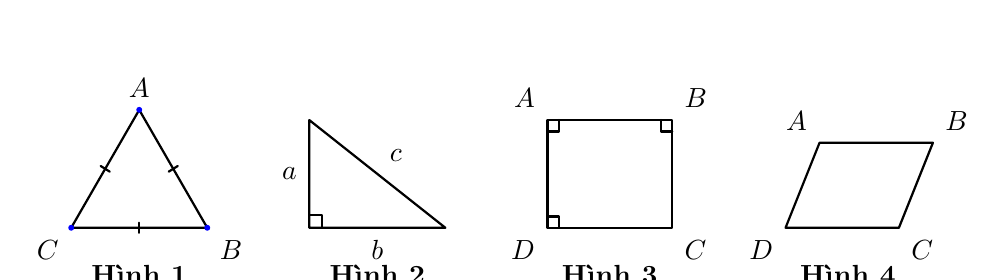
\begin{tikzpicture}[scale=0.72, line cap=round, line join=round]
    % Hình 1: Tam giác đều
    \begin{scope}[shift={(0,0)}]
        \coordinate (C) at (0,0);
        \coordinate (B) at (2.4,0);
        \coordinate (A) at (1.2, 2.08);
        \draw[thick] (A) -- (B) -- (C) -- cycle;
        \filldraw[blue] (A) circle (1.2pt) node[above=1pt, black] {$A$};
        \filldraw[blue] (B) circle (1.2pt) node[below right=1pt, black] {$B$};
        \filldraw[blue] (C) circle (1.2pt) node[below left=1pt, black] {$C$};
        % Ticks on sides
        \draw[thick] ($(A)!0.5!(B)+(-0.08,-0.05)$) -- ($(A)!0.5!(B)+(0.08,0.05)$);
        \draw[thick] ($(A)!0.5!(C)+(-0.08,0.05)$) -- ($(A)!0.5!(C)+(0.08,-0.05)$);
        \draw[thick] ($(B)!0.5!(C)+(0,-0.09)$) -- ($(B)!0.5!(C)+(0,0.09)$);
        \node[below=8pt] at (1.2,-0.1) {\textbf{Hình 1}};
    \end{scope}

    % Hình 2: Tam giác vuông
    \begin{scope}[shift={(4.2,0)}]
        \coordinate (D) at (0,0);
        \coordinate (E) at (2.4,0);
        \coordinate (F) at (0, 1.9);
        \draw[thick] (F) -- (D) -- (E) -- cycle;
        \draw[thick] (0, 0.22) -- (0.22, 0.22) -- (0.22, 0);
        \node[left=1pt] at ($(D)!0.5!(F)$) {$a$};
        \node[below=1pt] at ($(D)!0.5!(E)$) {$b$};
        \node[above right=1pt] at ($(F)!0.5!(E)$) {$c$};
        \node[below=8pt] at (1.2,-0.1) {\textbf{Hình 2}};
    \end{scope}

    % Hình 3: Hình chữ nhật
    \begin{scope}[shift={(8.4,0)}]
        \coordinate (D) at (0,0);
        \coordinate (C) at (2.2,0);
        \coordinate (B) at (2.2, 1.9);
        \coordinate (A) at (0, 1.9);
        \draw[thick] (A) -- (B) -- (C) -- (D) -- cycle;
        \draw[thick] (0, 0.2) -- (0.2, 0.2) -- (0.2, 0);
        \draw[thick] (0, 1.7) -- (0.2, 1.7) -- (0.2, 1.9);
        \draw[thick] (2.0, 1.9) -- (2.0, 1.7) -- (2.2, 1.7);
        \node[above left=1pt] at (A) {$A$};
        \node[above right=1pt] at (B) {$B$};
        \node[below right=1pt] at (C) {$C$};
        \node[below left=1pt] at (D) {$D$};
        \node[below=8pt] at (1.1,-0.1) {\textbf{Hình 3}};
    \end{scope}

    % Hình 4: Hình bình hành
    \begin{scope}[shift={(12.6,0)}]
        \coordinate (D) at (0,0);
        \coordinate (C) at (2.0,0);
        \coordinate (B) at (2.6, 1.5);
        \coordinate (A) at (0.6, 1.5);
        \draw[thick] (A) -- (B) -- (C) -- (D) -- cycle;
        \node[above left=1pt] at (A) {$A$};
        \node[above right=1pt] at (B) {$B$};
        \node[below right=1pt] at (C) {$C$};
        \node[below left=1pt] at (D) {$D$};
        \node[below=8pt] at (1.1,-0.1) {\textbf{Hình 4}};
    \end{scope}
\end{tikzpicture}
\end{center}
\choiceTF
{\True Hình 1 là tam giác đều vì có 3 cạnh bằng nhau}
{Trong Hình 2, hai cạnh $a$ và $b$ kề với góc vuông được gọi là hai cạnh huyền}
{\True Hình 3 là hình chữ nhật $ABCD$ có 4 góc ở các đỉnh đều là góc vuông}
{\True Hình 4 là hình bình hành $ABCD$ có hai cặp cạnh đối song song và bằng nhau}
\loigiai{
\begin{itemize}[leftmargin=0.6cm, itemsep=1pt]
\item \textbf{a)} \textbf{Đúng}. Hình 1 có 3 cạnh bằng nhau nên đây là tam giác đều.
\item \textbf{b)} \textbf{Sai}. Trong tam giác vuông ở Hình 2, hai cạnh $a$ và $b$ tạo thành góc vuông được gọi là hai cạnh góc vuông; cạnh $c$ đối diện với góc vuông mới là cạnh huyền.
\item \textbf{c)} \textbf{Đúng}. Hình 3 có 4 góc tại các đỉnh $A, B, C, D$ đều là góc vuông nên đây là hình chữ nhật $ABCD$.
\item \textbf{d)} \textbf{Đúng}. Hình 4 là hình bình hành $ABCD$, theo định nghĩa và tính chất của hình bình hành thì các cặp cạnh đối luôn song song và bằng nhau: $AB \parallel CD, AB = CD$ và $AD \parallel BC, AD = BC$.
\end{itemize}
}
\end{ex}


\setcounter{ex}{0}
\noindent\textbf{\large PHẦN III. CÂU HỎI TRẢ LỜI NGẮN}

\vspace{1mm}
\begin{ex}
Tìm số thực $x$, biết: $|x - 0{,}5| - \dfrac{1}{2} = 1{,}5$. \shortans{$x = 1{,}5$ hoặc $x = -0{,}5$}
\loigiai{
Ta có $|x - 0{,}5| = 1{,}5 + 0{,}5 = 2$? Đợi chút: đề bài là $|x - 1/2| - 1{,}5 = 0{,}5$ hay $|x - 0{,}5| - 1/2 = 1{,}5$?
Xem lại raw: $|x - 0{,}5| = 1{,}5 - 0{,}5 = 1$. Có hai trường hợp:
\begin{itemize}
    \item TH 1: $x - 0{,}5 = 1 \implies x = 1 + 0{,}5 = 1{,}5$.
    \item TH 2: $x - 0{,}5 = -1 \implies x = -1 + 0{,}5 = -0{,}5$.
\end{itemize}
Vậy $x = 1{,}5$ hoặc $x = -0{,}5$.

\textbf{Đáp số:} $x = 1{,}5$ hoặc $x = -0{,}5$
}
\end{ex}

\begin{ex}
Cho góc $\widehat{xOy} = 80^\circ$. Vẽ tia $Oz$ nằm giữa hai tia $Ox$ và $Oy$ sao cho $\widehat{xOz} = 30^\circ$. Gọi $Ot$ là tia phân giác của $\widehat{zOy}$. Tính số đo góc $\widehat{xOt}$. \shortans{$55^\circ$}
\loigiai{
Vì tia $Oz$ nằm giữa hai tia $Ox$ và $Oy$ nên:
\[ \widehat{xOz} + \widehat{zOy} = \widehat{xOy} \implies 30^\circ + \widehat{zOy} = 80^\circ \implies \widehat{zOy} = 50^\circ. \]
Vì $Ot$ là tia phân giác của góc $\widehat{zOy}$ nên:
\[ \widehat{zOt} = \dfrac{\widehat{zOy}}{2} = \dfrac{50^\circ}{2} = 25^\circ. \]
Vì tia $Oz$ nằm giữa hai tia $Ox$ và $Ot$ nên:
\[ \widehat{xOt} = \widehat{xOz} + \widehat{zOt} = 30^\circ + 25^\circ = 55^\circ. \]

\textbf{Đáp số:} $55^\circ$
}
\end{ex}


\setcounter{ex}{0}
\noindent\textbf{\large PHẦN IV. TỰ LUẬN}

\vspace{1mm}
\begin{ex}
Tính giá trị các biểu thức sau (tính bằng cách hợp lý nếu có thể):
\begin{enumerate}[label=\textbf{\alph*)}, leftmargin=0.8cm, itemsep=1pt]
\item $A = \left(-\dfrac{5}{7}\right) + \dfrac{2}{7} : \dfrac{2}{5}$;
\item $B = \dfrac{-5}{17} \cdot \dfrac{31}{33} + \dfrac{-5}{17} \cdot \dfrac{2}{33} + 2\dfrac{5}{17}$;
\item $C = \sqrt{16} + \sqrt{25} + \sqrt{36} + \sqrt{49}$;
\item $D = 0{,}(5) - 1\dfrac{1}{3} + 0{,}(7)$.
\end{enumerate}
\loigiai{
\textbf{a)} $A = -\dfrac{5}{7} + \dfrac{2}{7} \cdot \dfrac{5}{2} = -\dfrac{5}{7} + \dfrac{5}{7} = 0$.

\textbf{b)} $B = \dfrac{-5}{17} \cdot \left(\dfrac{31}{33} + \dfrac{2}{33}\right) + 2 + \dfrac{5}{17} = \dfrac{-5}{17} \cdot 1 + 2 + \dfrac{5}{17} = -\dfrac{5}{17} + \dfrac{5}{17} + 2 = 2$.

\textbf{c)} $C = 4 + 5 + 6 + 7 = 22$.

\textbf{d)} $D = \dfrac{5}{9} - \dfrac{4}{3} + \dfrac{7}{9} = \left(\dfrac{5}{9} + \dfrac{7}{9}\right) - \dfrac{4}{3} = \dfrac{12}{9} - \dfrac{4}{3} = \dfrac{4}{3} - \dfrac{4}{3} = 0$.
}
\end{ex}
\vspace{2mm}

\begin{ex}
Tìm $x$, biết:
\begin{enumerate}[label=\textbf{\alph*)}, leftmargin=0.8cm, itemsep=1pt]
\item $x + \dfrac{1}{2} = \dfrac{3}{4}$;
\item $\left|x - \dfrac{2}{3}\right| = \dfrac{1}{3}$.
\end{enumerate}
\loigiai{
\textbf{a)} $x = \dfrac{3}{4} - \dfrac{1}{2} = \dfrac{3}{4} - \dfrac{2}{4} = \dfrac{1}{4}$. Vậy $x = \dfrac{1}{4}$.

\textbf{b)} Ta có hai trường hợp:
\begin{itemize}
    \item TH 1: $x - \dfrac{2}{3} = \dfrac{1}{3} \implies x = \dfrac{1}{3} + \dfrac{2}{3} = 1$.
    \item TH 2: $x - \dfrac{2}{3} = -\dfrac{1}{3} \implies x = -\dfrac{1}{3} + \dfrac{2}{3} = \dfrac{1}{3}$.
\end{itemize}
Vậy $x = 1$ hoặc $x = \dfrac{1}{3}$.
}
\end{ex}
\vspace{2mm}

\begin{ex}
\immini{
Cho hình vẽ sau, trong đó $Ax \parallel By$, $\widehat{xAB} = 40^\circ, \widehat{ABC} = 105^\circ, \widehat{BCy} = 65^\circ$:
\begin{enumerate}[label=\textbf{\alph*)}, leftmargin=0.8cm, itemsep=1pt]
\item Tính số đo góc $\widehat{ABy}$.
\item Chứng minh rằng $By \parallel Cz$.
\item Kẻ $BD$ là tia phân giác của góc $\widehat{CBy}$ ($D \in Cz$). Tính số đo góc $\widehat{BDC}$.
\end{enumerate}
}{
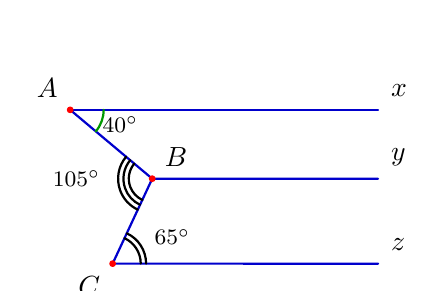
\begin{tikzpicture}[scale=0.85, line cap=round, line join=round]
    \coordinate (A) at (0, 2.2);
    \coordinate (Ax_end) at (4.6, 2.2);
    \coordinate (B) at ($(A)+({1.6*cos(-40)}, {1.6*sin(-40)})$);
    \coordinate (By_end) at (4.6, 1.171);
    \coordinate (C) at ($(B)+({-1.4*cos(65)}, {-1.4*sin(65)})$);
    \coordinate (Cz_end) at (4.6, -0.098);

    \draw[thick, blue!80!black] (A) -- (Ax_end) node[above right=1pt, black] {$x$};
    \draw[thick, blue!80!black] (B) -- (By_end) node[above right=1pt, black] {$y$};
    \draw[thick, blue!80!black] (C) -- (Cz_end) node[above right=1pt, black] {$z$};
    \draw[thick, blue!80!black] (A) -- (B) -- (C);

    \filldraw[red] (A) circle (1.2pt) node[above left=1pt, black] {$A$};
    \filldraw[red] (B) circle (1.2pt) node[above right=1pt, black] {$B$};
    \filldraw[red] (C) circle (1.2pt) node[below left=1pt, black] {$C$};

    % Angle xAB = 40 deg
    \draw[thick, green!60!black] (A) ++(0:0.5) arc (0:-40:0.5);
    \node[font=\footnotesize] at ($(A)+(0.75, -0.22)$) {$40^\circ$};

    % Angle ABC = 105 deg
    \draw[thick] (B) ++(140:0.35) arc (140:245:0.35);
    \draw[thick] (B) ++(140:0.43) arc (140:245:0.43);
    \draw[thick] (B) ++(140:0.51) arc (140:245:0.51);
    \node[font=\footnotesize, left=2pt] at ($(B)+(-0.55, 0)$) {$105^\circ$};

    % Angle BCz = 65 deg
    \draw[thick] (C) ++(0:0.42) arc (0:65:0.42);
    \draw[thick] (C) ++(0:0.5) arc (0:65:0.5);
    \node[font=\footnotesize, above right=2pt] at ($(C)+(0.4, 0.05)$) {$65^\circ$};
\end{tikzpicture}
}
\loigiai{
\textbf{a)} Vì $Ax \parallel By$ nên $\widehat{ABy} = \widehat{xAB} = 40^\circ$ (hai góc so le trong).

\textbf{b)} Tia $By$ nằm giữa hai tia $BA$ và $BC$ nên:
\[ \widehat{ABC} = \widehat{ABy} + \widehat{CBy} \implies 105^\circ = 40^\circ + \widehat{CBy} \implies \widehat{CBy} = 105^\circ - 40^\circ = 65^\circ. \]
Ta có $\widehat{CBy} = \widehat{BCz} = 65^\circ$. Mà hai góc này ở vị trí so le trong nên $By \parallel Cz$.

\textbf{c)} Vì $BD$ là tia phân giác của góc $\widehat{CBy}$ nên:
\[ \widehat{DBy} = \dfrac{\widehat{CBy}}{2} = \dfrac{65^\circ}{2} = 32{,}5^\circ. \]
Vì $By \parallel Cz$ nên $\widehat{BDC} = \widehat{DBy} = 32{,}5^\circ$ (hai góc so le trong).
}
\end{ex}
\vspace{2mm}

\begin{ex}
Cho $A = \dfrac{1}{7} + \dfrac{1}{7^2} + \dfrac{1}{7^3} + \dfrac{1}{7^4} + \ldots + \dfrac{1}{7^{2024}}$. Tìm $x$ để $6A = 1 - \dfrac{1}{7^x}$.
\loigiai{
Nhân cả hai vế của $A$ với $7$ ta được:
\[ 7A = 7 \cdot \left(\dfrac{1}{7} + \dfrac{1}{7^2} + \ldots + \dfrac{1}{7^{2024}}\right) = 1 + \dfrac{1}{7} + \dfrac{1}{7^2} + \ldots + \dfrac{1}{7^{2023}}. \]
Trừ từng vế $7A$ cho $A$:
\[ 7A - A = \left(1 + \dfrac{1}{7} + \ldots + \dfrac{1}{7^{2023}}\right) - \left(\dfrac{1}{7} + \dfrac{1}{7^2} + \ldots + \dfrac{1}{7^{2024}}\right) \]
\[ 6A = 1 - \dfrac{1}{7^{2024}}. \]
Theo đề bài: $6A = 1 - \dfrac{1}{7^x}$, suy ra:
\[ 1 - \dfrac{1}{7^{2024}} = 1 - \dfrac{1}{7^x} \implies \dfrac{1}{7^x} = \dfrac{1}{7^{2024}} \implies 7^x = 7^{2024} \implies x = 2024. \]
Vậy $x = 2024$.
}
\end{ex}
\vspace{2mm}


\begin{center}
\rule{4cm}{0.4pt}\\
\textit{--- HẾT ---}
\end{center}
\end{document}
